\documentclass[../nirs.tex]{subfiles}

\begin{document}
\section{Построение концептуальной и физической модели данных}
Основываясь на вышеперечисленные особенности разрабатываемой системы, была
создана концептуальная модель базы данных, изображенная на рисунке
\ref{fig:3_1_db_conceptual}.

\begin{figure}[H]
	\centering
	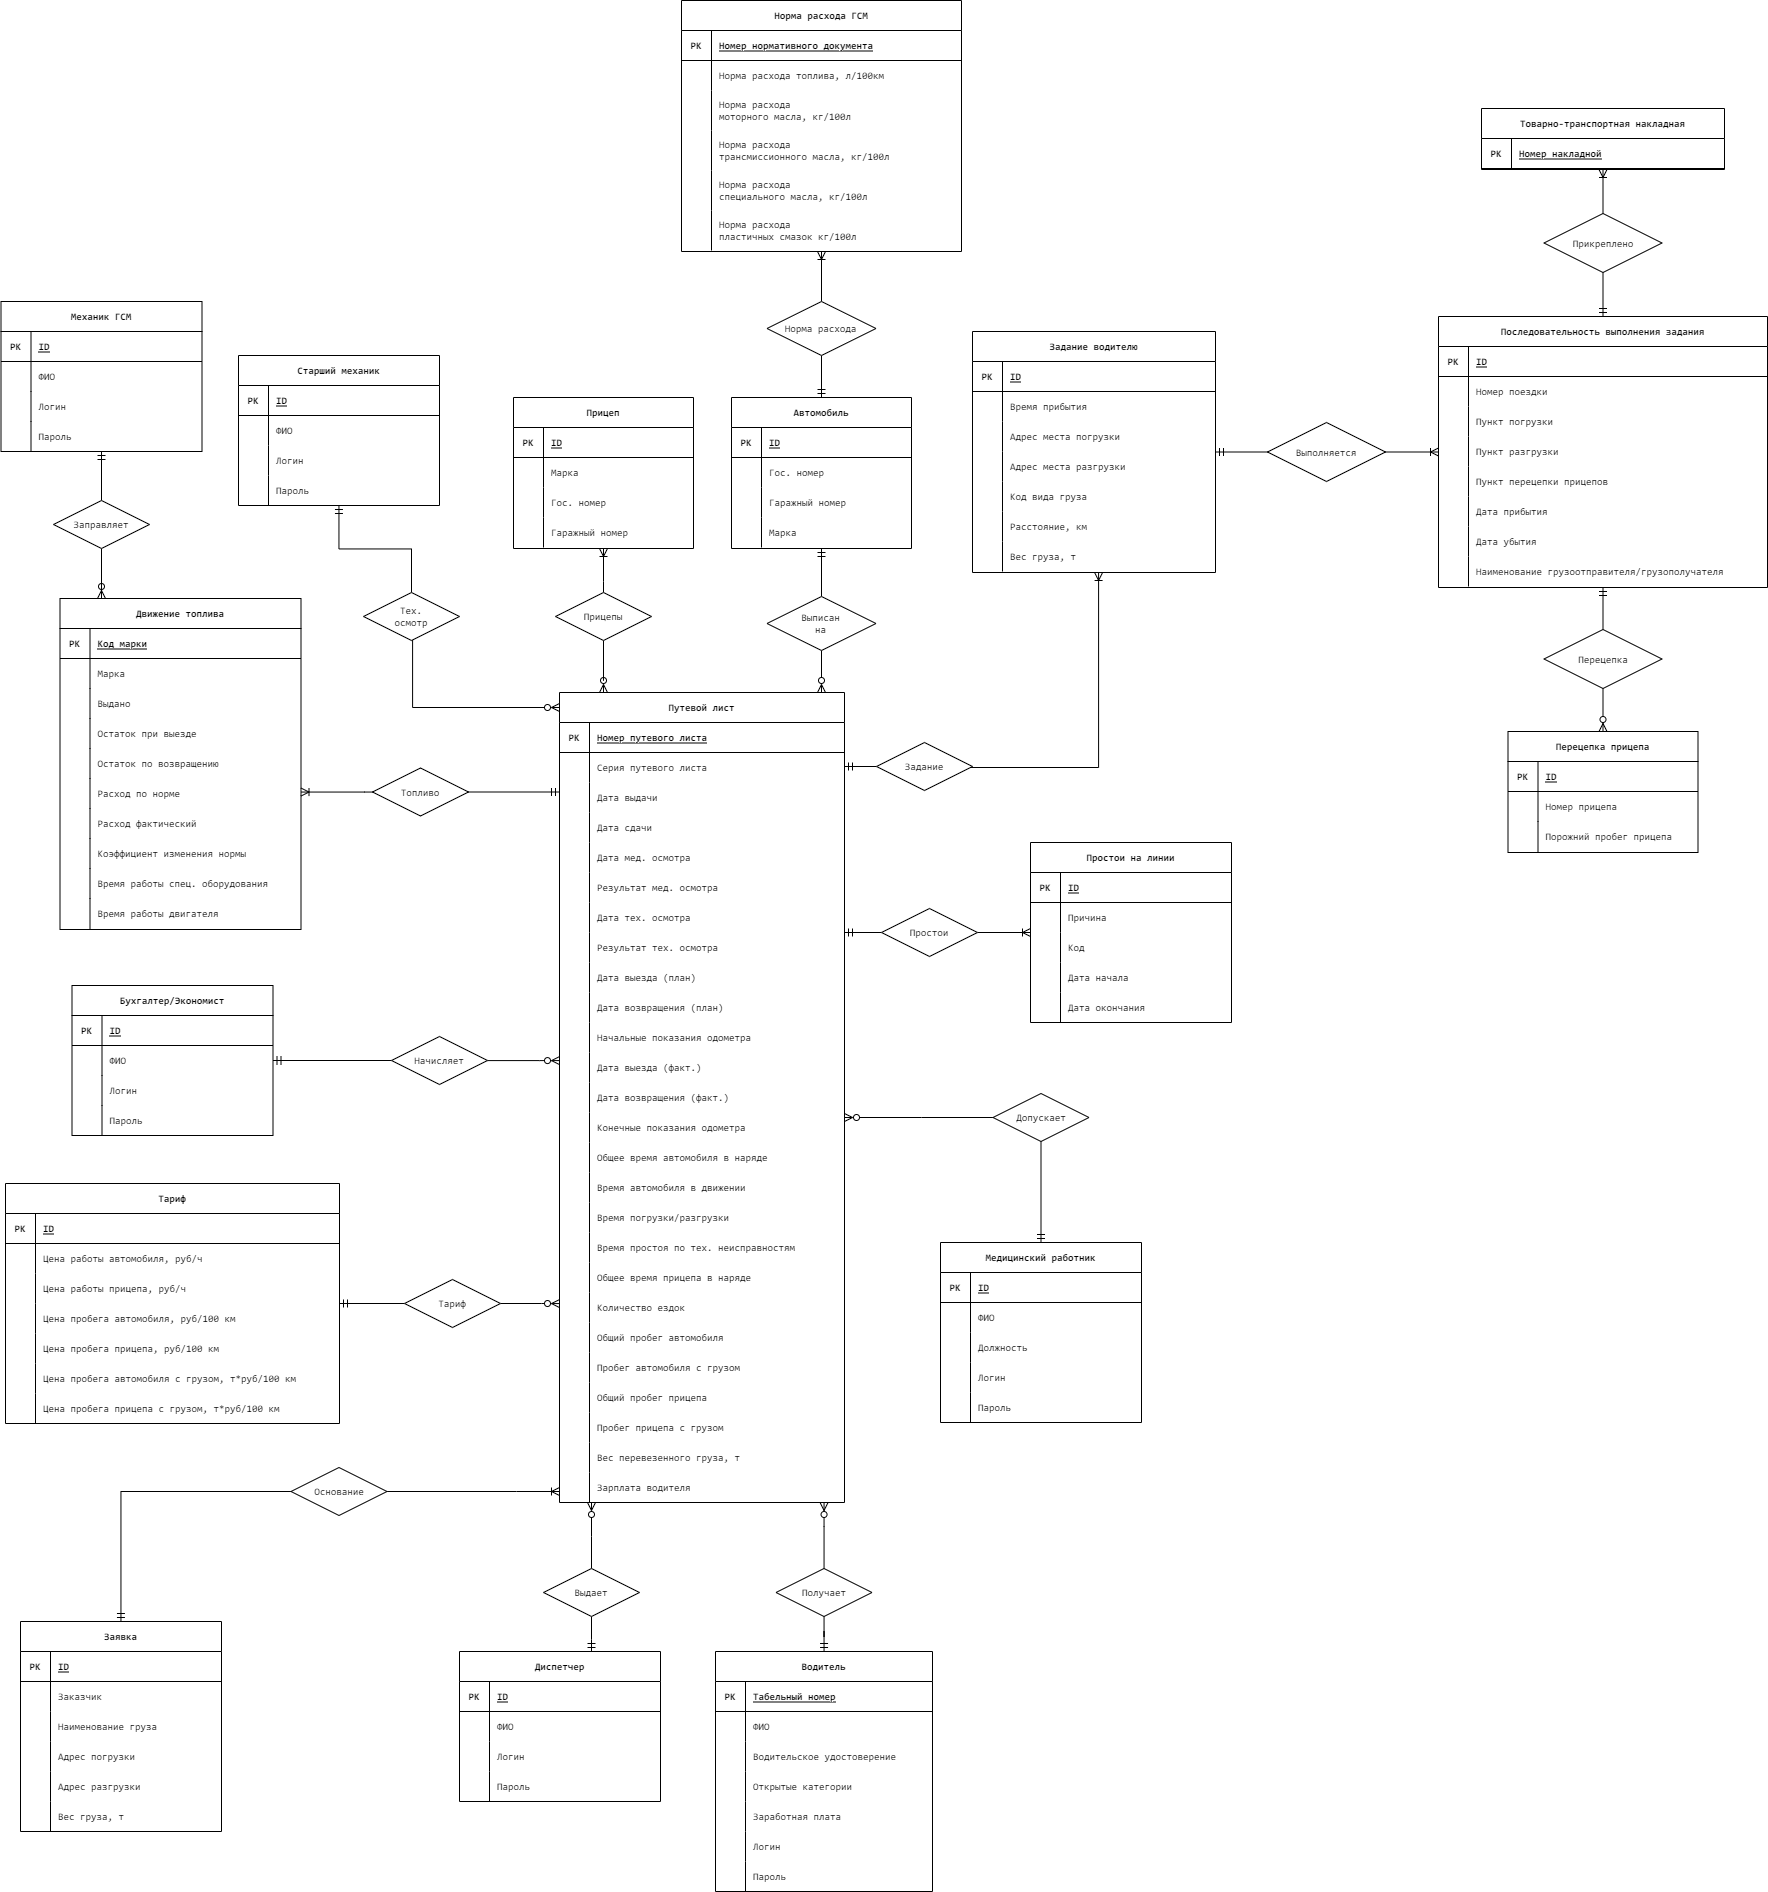
\includegraphics[keepaspectratio,width=\textwidth]{../2/images/2_1_3_er-diagram.png}
	\caption{Концептуальная модель данных разрабатываемой системы}
	\label{fig:3_1_db_conceptual}
\end{figure}

Концептуальная модель данных определяет смысловую структуру рассматриваемой
системы [8]. С ее помощью можно представить рассматриваемую предметную область
множеством сущностей и связей между ними. Каждая сущность обладает набором
свойств, именуемых атрибутами. Основная задача концептуальной модели -- передать
фундаментальное принципы и основные функциональные возможности проектируемой
системы [8].

Любая информационная система включает в себя некоторую систему управления базами
данных (СУБД). Концептуальная модель представления данных не подходит для
создания таблиц в реляционной СУБД. Чтобы можно было создать реляционную базу
данных необходимо концептуальную модель перевести в логическую, а затем в
физическую  модель данных, предназначенную для выбранной СУБД. На рисунке
\ref{fig:3_1_db_logical} представлена логическая модель данных разрабатываемой
системы.

\begin{figure}[H]
	\centering
	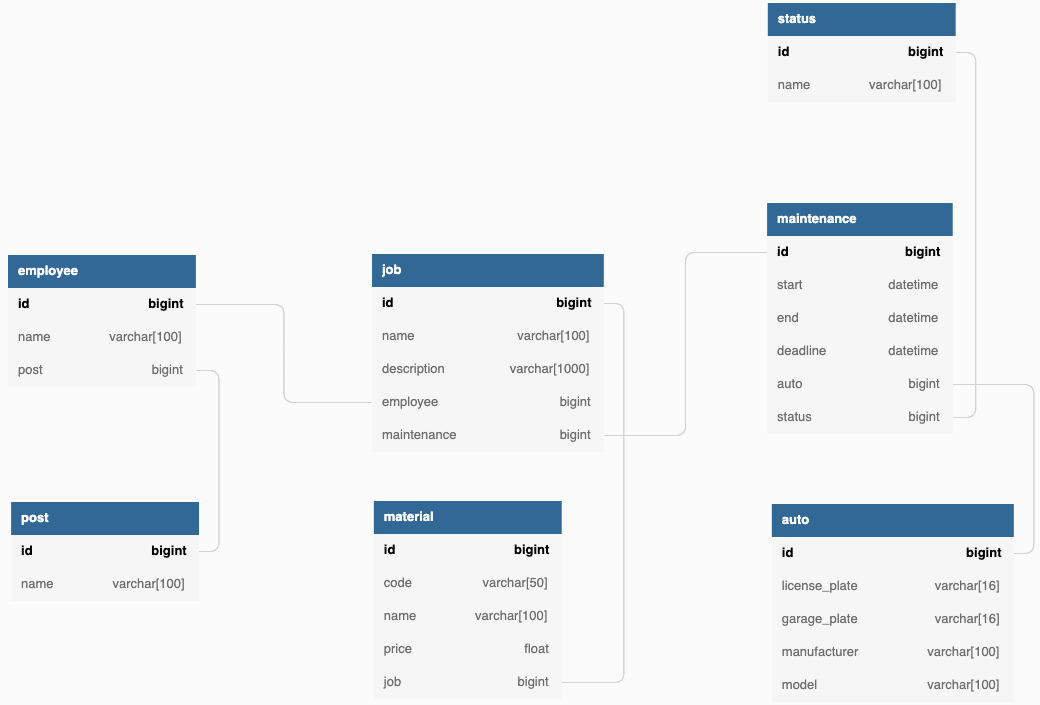
\includegraphics[keepaspectratio,width=\textwidth]{./images/3_1_db_physical.png}
	\caption{Логическая модель данных разрабатываемой системы}
	\label{fig:3_1_db_logical}
\end{figure}

Спецификация сущностей приведена в таблицах \ref{tab:waybills} --
\ref{tab:medical_workers}.
\subfile{tables/1_waybills.tex}
\subfile{tables/1_waybill_trailers.tex}
\subfile{tables/1_requests.tex}
\subfile{tables/1_price_lists.tex}
\subfile{tables/1_idle_times.tex}
\subfile{tables/1_fuel.tex}
\subfile{tables/1_task_conditions.tex}
\subfile{tables/1_autos.tex}
\subfile{tables/1_trailers.tex}
\subfile{tables/1_fuel_wasting.tex}
\subfile{tables/1_tasks.tex}
\subfile{tables/1_task_completions.tex}
\subfile{tables/1_consignment_notes.tex}
\subfile{tables/1_trailer_changes.tex}
\subfile{tables/1_user_types.tex}
\subfile{tables/1_users.tex}
\subfile{tables/1_drivers.tex}
\subfile{tables/1_medical_workers.tex}

\end{document}
